\section{Wichtige Funktionen im Zeitbereich}

\subsection[Einheitssprung]{Einheitssprung $\bm{u(t)}$}{17}

\begin{minipage}[c]{0.58\columnwidth}
    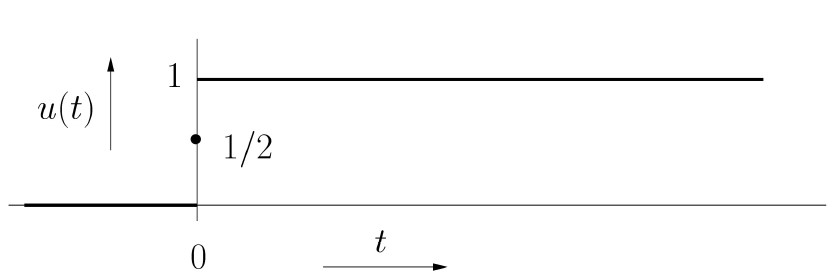
\includegraphics[width=\columnwidth]{images/einheitssprung.jpg}
\end{minipage}
\hfill
\begin{minipage}[c]{0.38\columnwidth}
    $$ u(t) = 
    \begin{cases}
        0           & \text{für } t < 0 \\
        \frac{1}{2} & \text{für } t = 0 \\
        1           & \text{für } t > 0
    \end{cases} $$
\end{minipage}


\subsection[Signumfunktion]{Signumfunktion $\bm{\sgn(t)}$}{18}

\begin{minipage}[c]{0.48\columnwidth}
    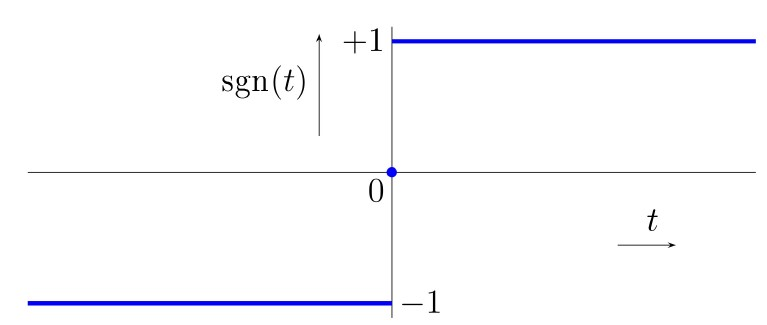
\includegraphics[width=\columnwidth]{images/signumfunktion.jpg}
\end{minipage}
\hfill
\begin{minipage}[c]{0.48\columnwidth}
    $$ \sgn(t) = 
    \begin{cases}
        -1  & \text{für } t < 0 \\
        0   & \text{für } t = 0 \\
        1   & \text{für } t > 0
    \end{cases} $$
\end{minipage}


\subsection[Rampenfunktion]{Rampenfunktion $\bm{r(t)}$}{18}

\begin{minipage}[c]{0.58\columnwidth}
    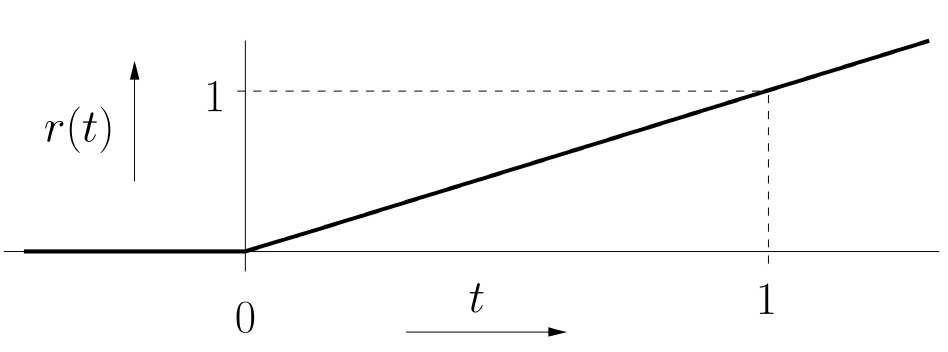
\includegraphics[width=\columnwidth]{images/rampenfunktion.jpg}
\end{minipage}
\hfill
\begin{minipage}[c]{0.38\columnwidth}
    $$ r(t) = 
    \begin{cases}
        0   & \text{für } t \leq 0 \\
        t   & \text{für } t > 0 
    \end{cases} $$
\end{minipage}


\subsection[Rechteckimpuls]{Rechteckimpuls $\bm{p_a(t)}$}{19}

\begin{minipage}[c]{0.58\columnwidth}
    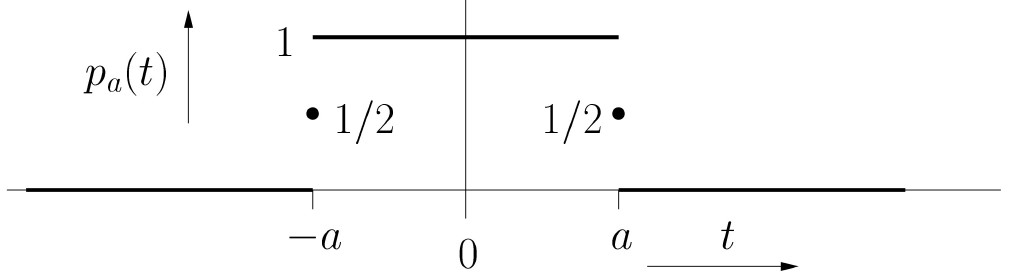
\includegraphics[width=\columnwidth]{images/rechteckimpuls.jpg}
\end{minipage}
\hfill
\begin{minipage}[c]{0.38\columnwidth}
    $$ p_a(t) = u(t+a) - u(t+a) $$
    $$ p_a(t) = 
    \begin{cases}
        1           & \text{für } \vert t \vert < a \\
        \frac{1}{2} & \text{für } \vert t \vert = a \\
        0           & \text{für } \vert t \vert > a 
    \end{cases} $$
\end{minipage}

\vspace{0.2cm}

Der Bereich von $-a$ bis $a$ heisst 'Support der Funktion'


\subsection[Dreieckimpuls]{Dreieckimpuls $\bm{\Lambda_a(t)}$}{20}

\begin{minipage}{0.5\columnwidth}
    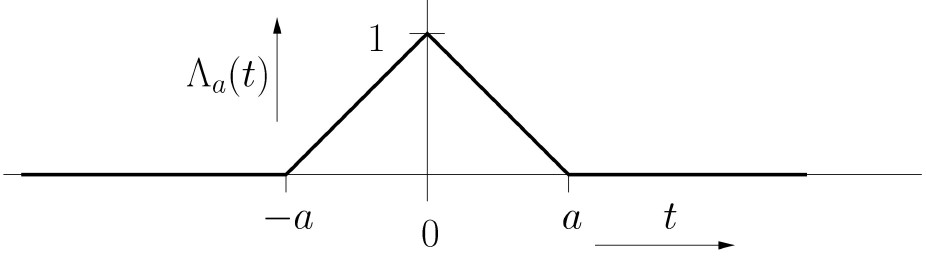
\includegraphics[width=\columnwidth]{images/dreieckimpuls.jpg}
\end{minipage}
\hfill
\begin{minipage}{0.48\columnwidth}
    $$ \Lambda_a(t) = 
    \begin{cases}
        1 - \frac{\vert t \vert}{a} & \text{für } \vert t \vert < a \\
        0                           & \text{für } |t| \geq a 
    \end{cases} $$
\end{minipage}

\vspace{0.2cm}

Der Bereich von $-a$ bis $a$ heisst 'Support der Funktion'


\subsection[Sincfunktion]{Sincfunktion $\bm{\mathrm{sinc}(t)}$}{20}

\begin{minipage}{0.48\columnwidth}
    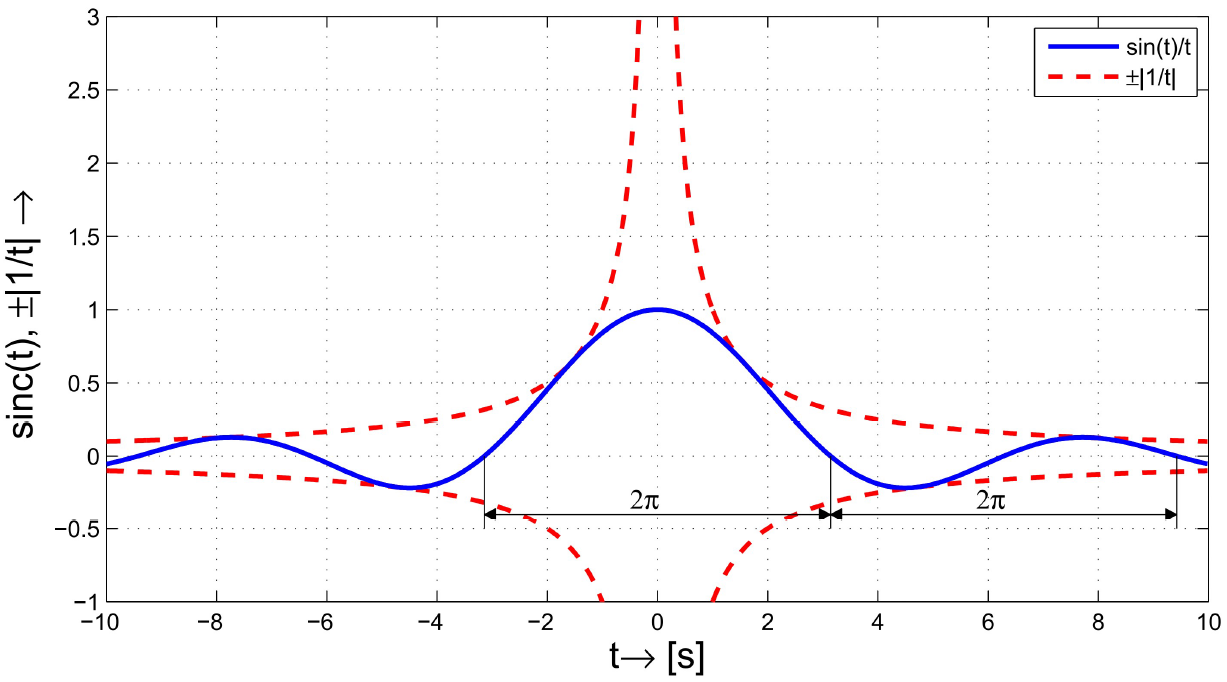
\includegraphics[width=\columnwidth]{images/sinc_funktion.png}
\end{minipage}
\hfill
\begin{minipage}{0.48\columnwidth}
    $$ \mathrm{sinc}(t) = \frac{\sin(t)}{t} \, \forall  \, t $$
\end{minipage}


\subsection[Deltafunktion (Dirac-Stoss)]{Deltafunktion (Dirac-Stoss) $\bm{\delta(t)}$}{21-23}

\begin{minipage}{0.58\columnwidth}
    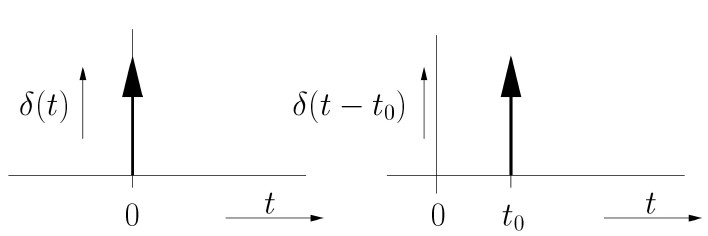
\includegraphics[width=\columnwidth]{images/deltafunktion.jpg}
\end{minipage}
\hfill
\begin{minipage}{0.38\columnwidth}
    $$ \delta(t) = 
    \begin{cases}
        \infty  & \text{für } t = 0 \\
        0       & \text{sonst}
    \end{cases} $$
        
    $$ \int\limits_{- \infty}^{\infty} \delta(t) \, \diff t = 1 $$
\end{minipage}


\subsubsection{Eigenschaften der Delta-Funktion}

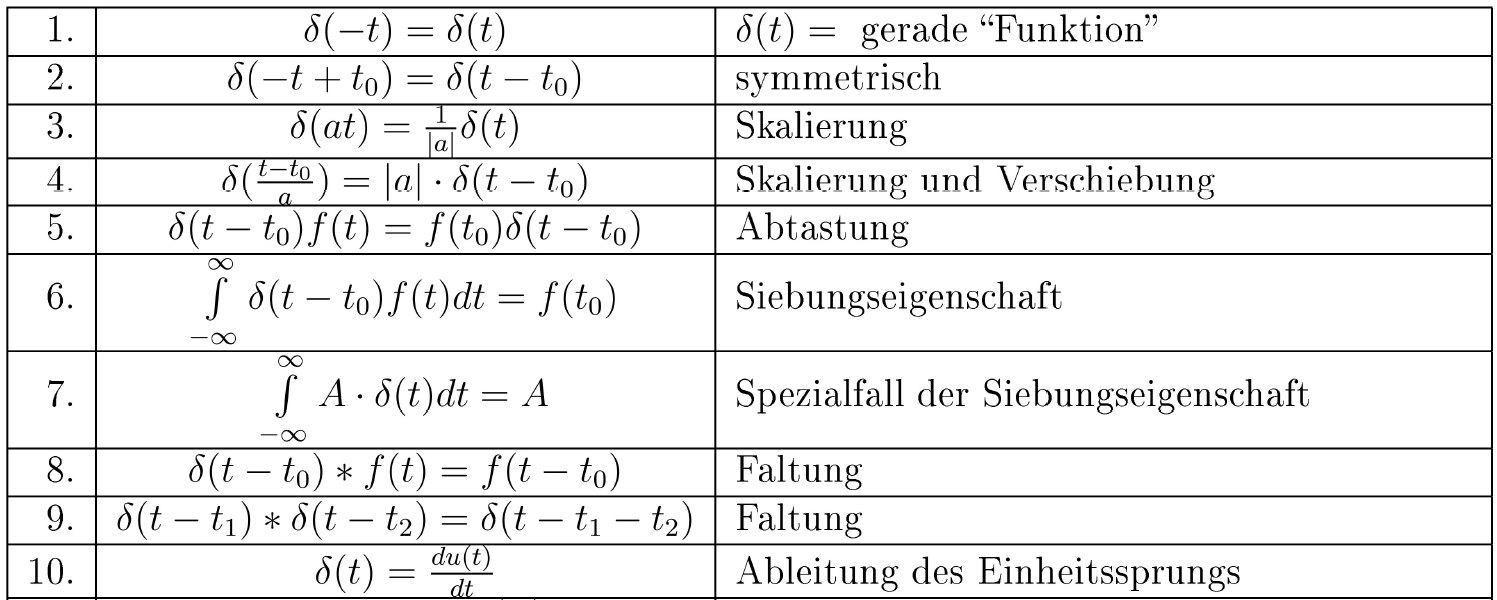
\includegraphics[width=\columnwidth]{images/eigenschaften_dirac_reduziert.png}

\vspace{0.2cm}

\textbf{\textrightarrow\ Skript S.22}


\subsection{Signalmanipulationen}{23-24}

% Von Analysis 1a Zusammenfassung

\begin{tabular}{lll}
    1.  & Streckung um $\bm{\frac{1}{a}}$ in $x$-Richtung               & $y = f(a \cdot x)$    \\
        & Spiegelung an $y$-Achse bei $\bm{-a}$ \\
    2.  & Verschiebung nach links ($\bm{+b}$) oder rechts ($\bm{-b}$)   & $y = f(x \pm b)$      \\
    3.  & Streckung um $\bm{c}$ in $y$-Richtung                         & $y = c \cdot f(x)$    \\
        & Spiegelung an $x$-Achse bei $\bm{-c}$ \\
    4.  & Verschiebung nach oben ($\bm{+d}$) oder unten ($\bm{-d}$)     & $y = f(x) \pm d $ 
\end{tabular}


\subsection{Rauschen}{25}

Rauschen bezeichnet die unregelmässige Bewegung von Ladungsträgern, welche eine Rauschspannung zur Folge hat. \\
Ist die Intensität der Rauschspannung über viele Frequenzdekaden gleich verteilt, so spricht man von weissem Rauschen.

\vspace{0.2cm}

\begin{tabular}{ll}
    \textbf{Weisses Rauschen}   & \textbf{Konstante Rauschleistung für alle Frequenzen} \\
    Farbiges Rauschen           & Frequenzabhängige Rauschleistung 
\end{tabular}

\vspace{0.2cm}

Ein \textbf{Rauschsignal} ist ein \textbf{Störsignal}, welches sich zum Nutzsignal addiert und dieses dadurch verfälscht.


\subsection{Thermisch bedingtes Rauschen (Widerstände)}

Folgende beiden Gleichungen gelten für Frequenzen bis ca. $3 \cdot 10^{12} \, \hertz$

\vspace{0.2cm}

\begin{tabular}{lll}
    $T$         & \textbf{Absolute} Temperatur                                                  & $[T] = \kelvin$                   \\
    $\Delta f$  & Bandbreite                                                                    & $[\Delta f] = \hertz$             \\
    $k$         & Boltzmann-Konstante $k = 1.380662 \cdot 10^{-23} \, \frac{\joule}{\kelvin}$   & $[k] = \frac{\joule}{\kelvin}$ 
\end{tabular}


\subsubsection{Effektive Rauschleistung $P_r$}

\vspace{-0.2cm}
$$  \boxed{ P_r = k \cdot T \cdot \Delta f } $$


\subsubsection{Effektive Rauschspannung $U_r$}

\vspace{-0.2cm}
$$  \boxed{ U_r = \sqrt{ 4 \cdot k \cdot T \cdot \Delta f \cdot R } } $$



\subsection[Signal-Rausch-Verhältnis (SNR)]{Signal-Rausch-Verhältnis (SNR) $\bm{a_r}$}{27}

Das Signal-Rausch-Verhältnis wird auch Störabstand oder Rauschabstand $a_r$ genannt. \\
Das SNR dient zur \textbf{Qualitätsbewertung von Signalen} 

$$ \boxed{ a_r = 10 \cdot \log \left( \frac{P_s}{P_r} \right) = 20 \cdot \log \left( \frac{U_s}{U_r} \right) } $$

\begin{tabular}{lll}
    $a_r$   & Störabstand / Rauschabstand / SNR     & $[a_r] = \deci \bel$  \\
    $P_s$   & Leistung des Nutzsignals              & $[P_s] = \watt$       \\
    $P_r$   & Leistung des Rauschsignals            & $[P_r] = \watt$       \\
    $U_s$   & Effektive Rauschspannung              & $[U_s] = \volt$       \\
    $U_r$   & Effektive Rauschleistung              & $[U_r] = \volt$
\end{tabular}


\subsubsection{Rauschzahl (noise figure) $F$}

Jeder Vierpol in einer Verstärkerkette (Serieschaltung) fügt dem Rauschen an seinem Eingang ein zusätzliches Rauschen hinzu. \\
Der \textbf{ausgangsseitige Rauschabstand} wird so \textbf{verkleinert}.

$$ \boxed{ F = \frac{\frac{P_{s \,\text{Eingang}}}{P_{r \,\text{Eingang}}}}{\frac{P_{s \,\text{Ausgang}}}{P_{r \,\text{Ausgang}}}}
    = \frac{P_{s \,\text{Eingang}}}{P_{r \,\text{Eingang}}} \cdot \frac{P_{r \,\text{Ausgang}}}{P_{s \,\text{Ausgang}}} } $$

Eine Rauschzahl von $F = 1$ ergibt sich einem einem \textbf{idealen Vierpol}


\subsubsection{Rauschmass $\bm{a_F}$}

Das Rauschmass $a_F$ ist die logarithmische Darstellung der Rauschzahl $F$

$$ \boxed{ a_F = 10 \cdot \log(F) = a_{r \,{\text{Eingang }}} - a_{r \,{\text{Ausgang }} } } $$ 

